\chapter{Toy example - the box model}
This chapter describes the inversion of a simple toy example with IFOS3D, which is a subdivided box in a homogeneous full space. This example can be performed as a first synthetic application to test IFOS3D on your system. The necessary input files and scripts are included in the IFOS3D folders and you can follow the following guidelines to perform a successfull inversion.  Your results can be compared to those given in this chapter.\\
The 3D inversion is costly even for a simple model. To enable a successfull inversion we therefore recommend the use of a  parallel system with a larger number of CPU's as for example found in supercomputing centers. We performed this inversion using 512 CPU's for 7.5 hours. Before starting this toy example, IFOS3D needs to be installed on your system (see chapter~\ref{Gettingstarted}).
\section{Inversion setup}
\subsection{Model and grid system}
\begin{figure}[h!]
\begin{center}
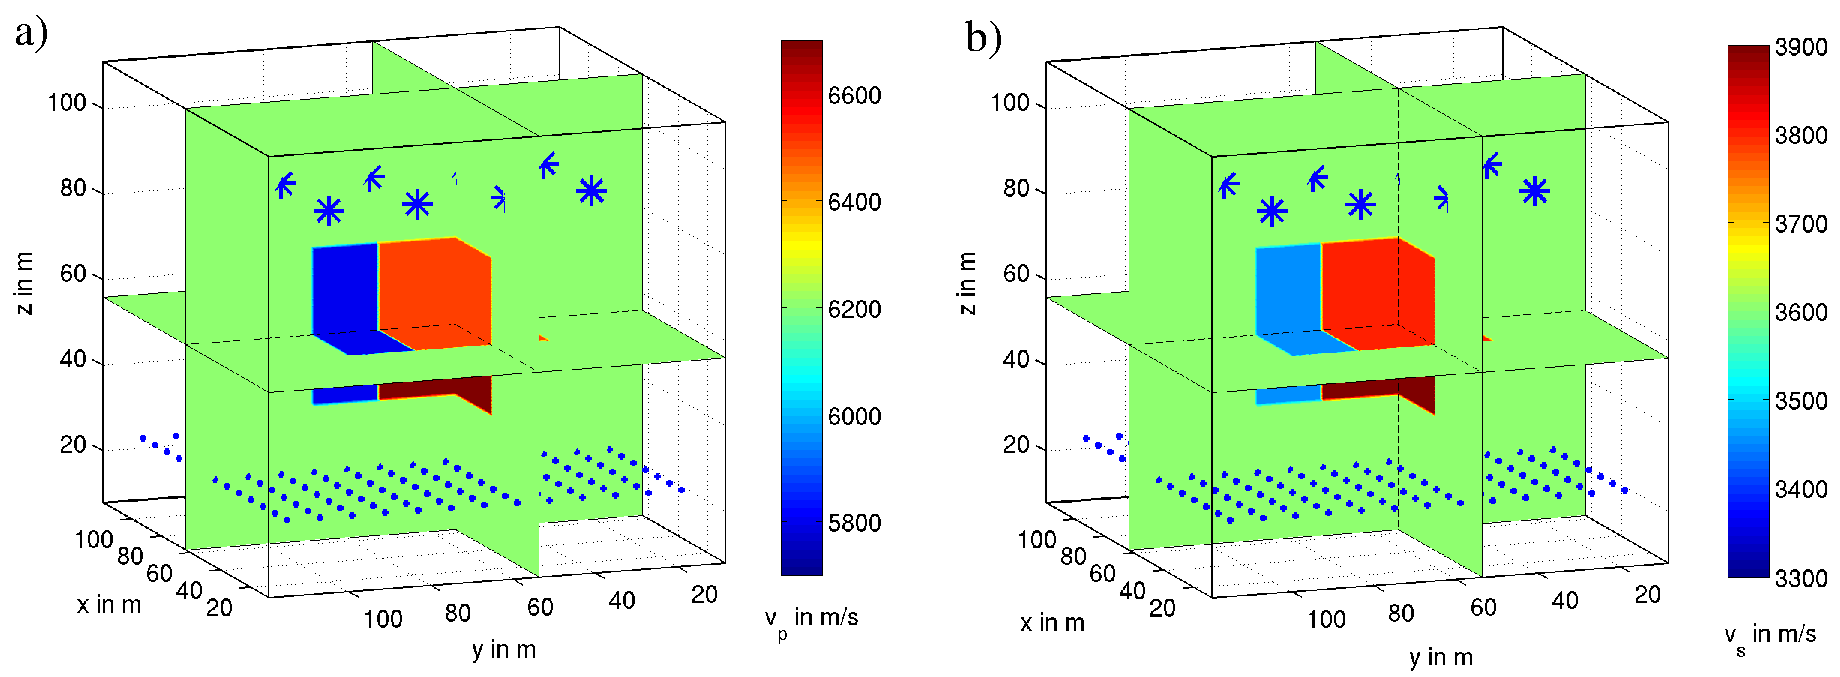
\includegraphics[width=\textwidth]{fig_toy/toy_real_model}
\caption[Toy example - the real model and acquisition geometry]{The toy example - real model $v_p$ (a) and $v_s$ (b), sources and receivers indicated as stars and crosses, respectively}\label{fig:toy_model}
\end{center}
\end{figure}
The true model for the seismic velocities is plotted in figure~\ref{fig:toy_model}. A box divided into four differently-sized parts with different positive and negative velocity variations is placed into a homogeneous full space of $v_p=6200$\,m/s and $v_s=3600$\,m/s. The $v_p$/$v_s$ ratio is not constant.
The density model is homogeneous with 2800\,kg/m$^3$ and kept constant during inversion. The elastic model is generated in IFOS3D on the fly (\textbf{READMOD}=0) using the function \textit{src/hh\_toy.c} as defined in \textit{src/Makefile}.\\
The model size is 128\,m$\times$128\,m $\times$147.2\,m in $x$-, $y$- and $z$-direction. We use a grid point distance of \textbf{DX}=\textbf{DY}=\textbf{DZ}=0.8\,m and thus a grid size of \textbf{NX}=160, \textbf{NY}=160 and \textbf{NZ}=184 points. \\
We use spatial FD-operators of \textbf{FDORDER}=4 and Holberg coefficients (\textbf{FDCOEFF=2}). This fullfills the dispersion criterion (see SOFI manual) up to a frequency of 500\,Hz ($v_{s,min}=3450$\,m/s):
\begin{equation}
 dh <= \frac{v_{s,min}}{nf_{max}}=\frac{v_{s,min}}{8.32f_{max}}
\end{equation}
For our maximum frequency of 320\,Hz used for inversion this is well sufficient. \\
The total calculation time is \textbf{TIME}=0.06\,s with a time stepping of 5e$^{-5}$s resulting in 1200 tiesteps per forward modeling. The stability criterion is fullfilled ($v_{p,max}=6700$\,m/s):
\begin{equation}
 dt<=\frac{dh}{0.487v_{p,max}}=2.4e^{-4}
\end{equation}
The model does not contain a free surface (\textbf{FREE\_SURF}=0) and as boundary condition we use a PML-layer (\textbf{FW}) of 10 grid points width at each model side.\\
\subsection{Sources and receivers}
\begin{figure}[h!]
\begin{center}
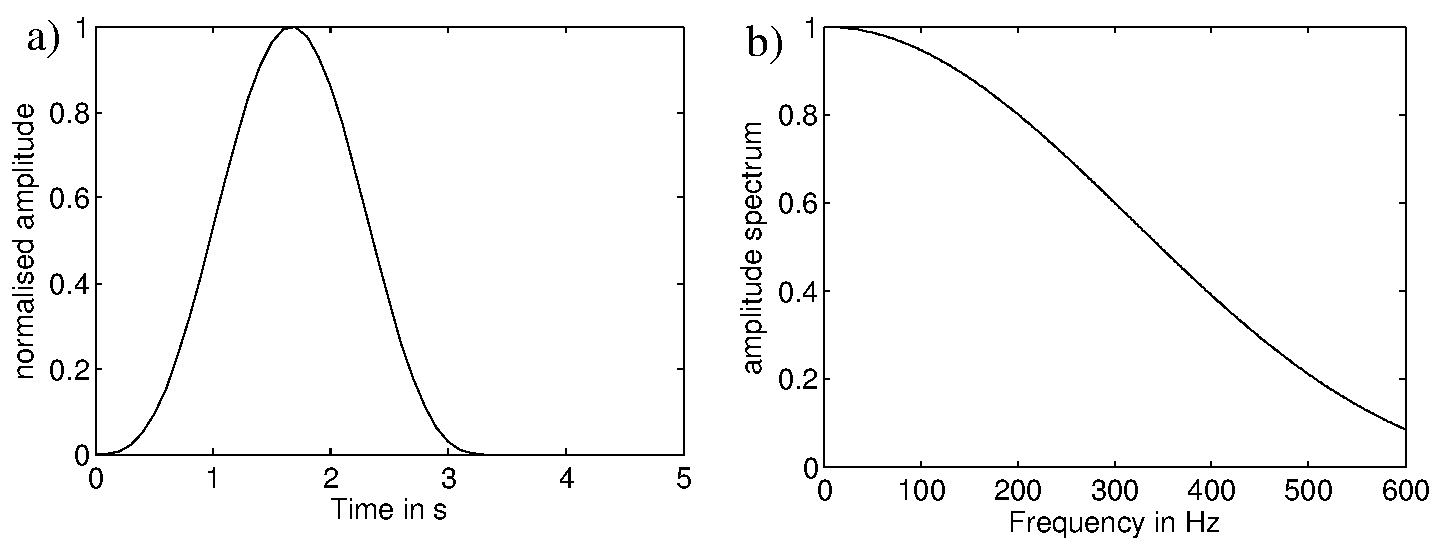
\includegraphics[width=0.8\textwidth]{fig_toy/source_toy}
\caption[Toy example - source wavelet and spectrum]{The toy example - normalised amplitude and spectrum of sin$^3$-source wavelet }\label{fig:toy_wavelet}
\end{center}
\end{figure}
Sources and receivers are arranged within $x$-$y$-planes, as indicated in Figure~\ref{fig:toy_model}. The sources are listed in \textit{sources/sources\_toy.dat} (\textbf{SOURCE\_FILE}). We use 12 (3$\times$4) sources in 92\,m depth with a central frequency of \textbf{FC}=300\,Hz. The sources are vertical directed point forces (\textbf{QUELLTYP}=4) with sin$^3$-wavelets (\textbf{QUELLART=4}) as source time functions. The corresponding source wavelet can be seen in figure~\ref{fig:toy_wavelet}a. This source wavelet comprises the low frequencies with $40\%$ of the maximum amplitude left at about 400\,Hz (figure~\ref{fig:toy_wavelet}b). \\
The receivers are arranged using a horizontal receiver array (\textbf{REC\_ARRAY}=1) in 24\,m depth. The distance between the receivers is \textbf{DRX}=\textbf{DRY}=10 gridpoints, which gives a total number of 169 receivers. 
\subsection{Inversion parameters}
For the inversion we use homogeneous starting models with $v_s=3600$\,m/s and $v_p=6200$\,m/s. In total 60 iterations are performed (\textbf{ITMIN, ITMAX }= 1, 60) and five frequencies are employed simultanously (\textbf{NFMAX}=5). For preconditioning of gradients a local taper is applied around source and receiver positions (\textbf{DAMPTYPE}=2). We do not use the diagonal Hessian approximation (\textbf{HESS}=0) or the L-BFGS method (\textbf{LBFGS}=0). Out of the total number of 12 shots we use 4 shots for the steplength estimation (\textbf{NSHOTS\_STEP}=4) and start with an initial test steplength of 0.02 (\textbf{TESTSTEP}=0.02). The filenames for gradient and model output are given in the input file.
\subsubsection*{The workflow}
The workflow file \textit{in\_and\_out} defines the different frequency stages. They are listed in table~\ref{tab:toy_fstage}.\\
\begin{table}[h!]
\centering 
\begin{tabular}{|c|c|c|c|}\hline
 iteration& frequencies in Hz & $\lambda_{min}(v_p)$ in m &$\lambda_{min}(v_s)$ in m \\
 1-15& 160,170,180,190,200 & 31 & 18\\
16-30& 200,210,220,230,240 & 26 & 15\\
31-45& 240,250,260,270,280 & 22 & 13\\
46-60& 280,290,300,310,320 & 19 & 11\\
\hline
\end{tabular}
\caption[Transmission example: frequency stages]{Frequency stages used for the transmission geometry box example with minimum wavelengths $\lambda_{min}(v_p)$ and $\lambda_{min}(v_s)$.}
\label{tab:toy_fstage}
\end{table}
We used four frequency stages with five frequencies, which increase from stage to stage. The frequency bands are slightly overlapping. The table  also lists the ninimum and maximum wavelengths, which define the resolution of the result. In the first stage lower frequencies enable the reconstruction of rough model structures, whereas higher frequencies and smaller wavelengths result in a higher resolution of smaller model structures.
\section{Step by step guideline}
\subsection{Step 1 - forward modeling}
In a first step, a forward modeling is performed to calculate data of the box model, which can be used as observed data in the inversion. This corresponds to a SOFI3D simulation. The model is created on the fly by the function \textit{src/hh\_toy.c}. The parameters are already set in \textit{in\_and\_out/ifos3D\_toy.inp}. For the forward modeling we use \textbf{METHOD}=0. The seismograms are written in the folder \textit{su\_obs}. For the option \textbf{METHOD}=0 the seismograms are written in one file for each processor containing receiver locations. From these files the data can be directly used as input in the inversion. Note, that \textbf{FILT}=0 and the program calculates the unfiltered seismograms. The box model is saved in the folder \textit{model}.\\
To perform the modeling the following steps are applied:
\begin{itemize}
 \item compile IFOS3D (execute \textit{./compileIFOS3D.sh})
 \item adapt processor number in \textit{in\_and\_out/ifos3D\_toy.inp} and your job script (e.g. \textit{startIFOS3D.sh})
 \item start IFOS3D (e.g. execute \textit{./startIFOS3D.sh})
\end{itemize}
The progress of IFOS3D can be viewed in \textit{in\_and\_out/ifos3D\_toy.out}. 
\subsection{Step 2 - the FWI}
In a second step, the inversion is performed. Before staring the inversion perform the following steps:
\begin{itemize}
 \item set the parameter (kasten=0) in \textit{src/hh\_toy.c} to gain homogeneous starting models
 \item compile IFOS3D (execute \textit{./compileIFOS3D.sh})
 \item change the following parameters in \textit{in\_and\_out/ifos3D\_toy.inp}: \textbf{METHOD}=1, \textbf{FILT}=1, \textbf{SEIS\_FILE} = ./su/cal\_toy
 \item start IFOS3D (e.g. execute \textit{./startIFOS3D.sh})
\end{itemize}
Now the inversion is performed. The proceedings of IFOS3D can be seen in the outputfile \textit{in\_and\_out/ifos3D.out}. An overview how the inversion succeeds, e.g. misfit values and steplengths can be found in the output file \textit{in\_and\_out/ifos3D\_invers.out}. Both files are written during simulation.
\section{Results}
In this section we look at the output of IFOS3D and show the inversion results. All output is located in the folder \textit{par}. For processing and plotting of data we use Matlab programs, located in the folder \textit{mfiles} and Seismic Unix.
\subsection{Seismograms}
\subsubsection*{Output}
The observed seismograms are calculated in step 1- forward modeling. They are located in the folder \textit{su\_obs} and provide unfiltered particle velocities for each shot and component in the su-format (e.g. \textit{obs\_toy\_vx\_it1.su.shot3}). \\
The inverted seisograms are stored in each iteration for each shot and each component in the folder \textit{su}. They are also in the su-format and named for instance \textit{cal\_toy\_vy\_it30.su.shot2}. Note that these data are filtered below the highest frequency used within the corresponding frequency stage.\\
The su-header in front of each trace contains i.a. information about source and receiver location, time stepping and time samples. It can be viewed using the Seismic Unix function \textit{surange} $<$ FILENAME or the Matlab function \textit{su2matlab}. 
\subsubsection*{Data plot}
For a first look, the seismograms can be plotted with the SU-routine \textit{suxwigb} $<$ FILENAME. Note, that it can be necessary to use the function \textit{segyclean} $<$ FILENAME $>$ FILENAME\_OUT before plotting.\\
For a comparison of obeserved and inverted data, it is necessary to apply a lowpass filter to the observed data, using the maximum frequency of the corresponding stage. Figure~\ref{fig:toy_seismo1} shows a comparison between initial, observed and inverted seismograms for one source and receiver and $x$-, $y$- and $z$-component of the particle velocity. Note, that the observed data was filtered with the maximum frequency of the first iteration for a comparison in a) and with the maximum inversion frequency for a comparison with the final inverted data in b). The plot was produced with the Matlab program \textit{seismo\_trace\_toy.m}. This program uses the binary format as input, which is why the files need to be transformed before use, applying the SU-routine \textit{sustrip} $<$ FILENAME $>$ FILENAME\_OUT.
\begin{figure}[h!]
\begin{center}
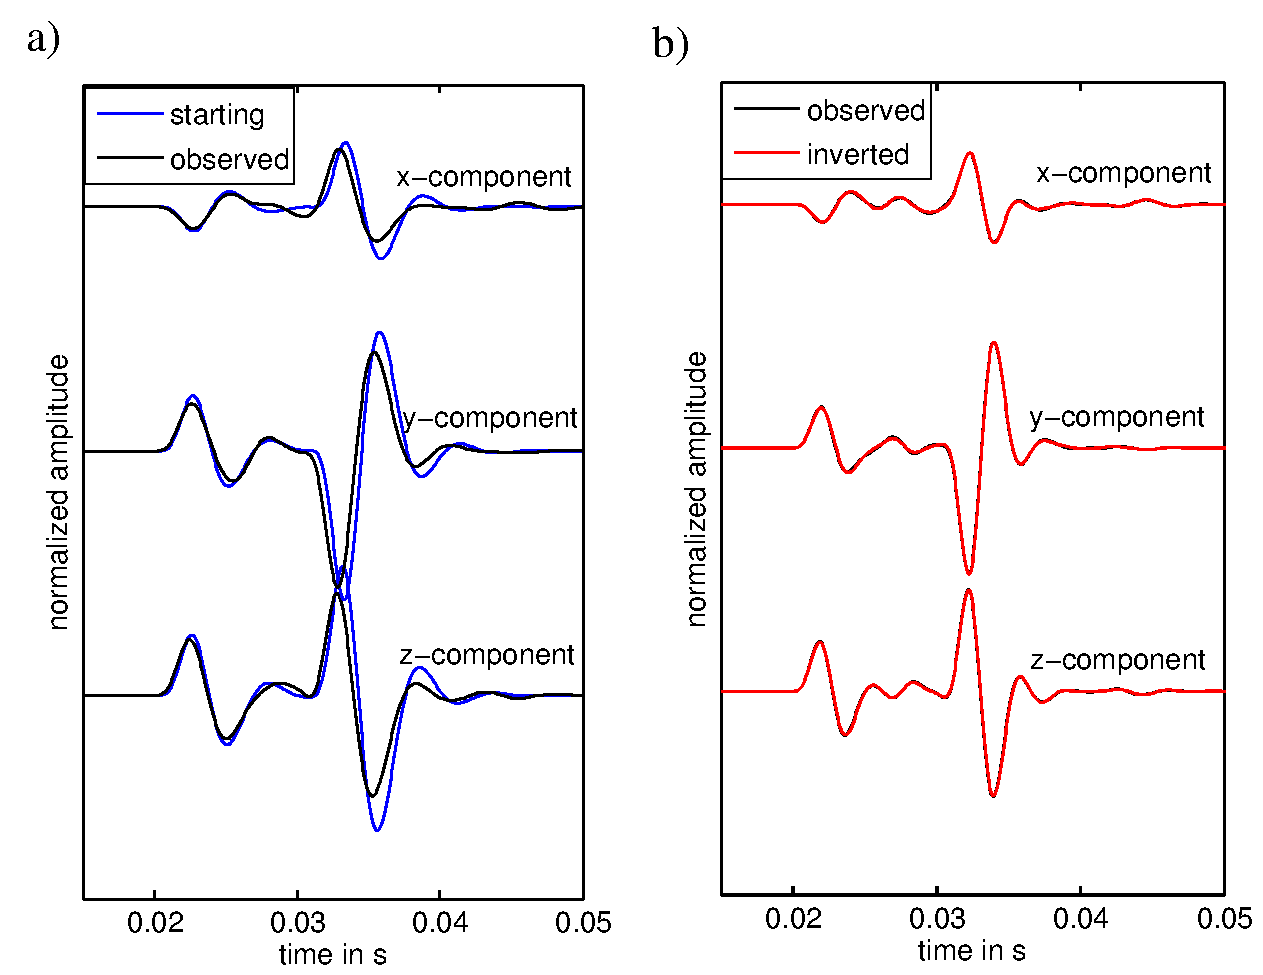
\includegraphics[width=\textwidth]{fig_toy/seismo1_toy}
\caption[Toy example - observed, initial and inverted seismograms]{Multi-component seismograms exemplarily for source at ($x_s$, $y_s$, $z_s$) = (32\,m, 96\,m, 92\,m) and receiver at ($x_r$, $y_r$, $z_r$) = (56\,m, 40\,m, 24\,m), normalised to one trace a) initial vs. observed data filtered below 200\,Hz and b) observed vs. inverted data filtered below 320\,Hz} \label{fig:toy_seismo1}
\end{center}
\end{figure}
\subsubsection*{Discussion}
Figure~\ref{fig:toy_seismo1} shows the comparison of initial and observed data for the low frequencies of the first inversion stage. The waveforms show only small differences and clearly no cycle skipping. Thus the homogeneous starting model is already sufficient for this simple example. \\
The success of the inversion can be seen when comparing the observed and inverted data. The waveforms, including the small oscillations are fitted very well for all components.
\subsection{The gradient} 
Gradients for $v_p$, $v_s$ and $\rho$ are stored in binary format in each iteration in the folder \textit{grad} (e.g. \textit{toy\_grad.vp\_200.00Hz\_it5}). Additionally to the raw gradients named by iteration number, the conjugate gradients are stored with labels of (iteration number +1000), like  (e.g. \\ \textit{toy\_grad.vp\_200.00Hz\_it1005}). \\
The gradients can be plotted with the Matlab program \textit{slice\_3D\_toy\_grad.m}. This program plots the 3D grid as two perpendicular slices. The acquisition geometry of the toy example is also included. \\
Here, we show the ``raw'' gradients and the preconditioned gradients of $v_p$ and $v_s$ normalised to their maximum value for the first iteration (figure~\ref{fig:toy_grad}). In the raw gradients (a,b) the high amplitudes around sources and receivers are clearly visible. Especially the source artefacts are very distinct compared to the small scaled receiver artefacts. By preconditioning these artefacts can be removed for the greater part (c,d) and the main update concentrates on the box area. Due to the smaller wavelengths of the shear wave, the $v_s$-gradient already shows more structure than the $v_p$-gradient. 
\begin{figure}[h!]
\begin{center}
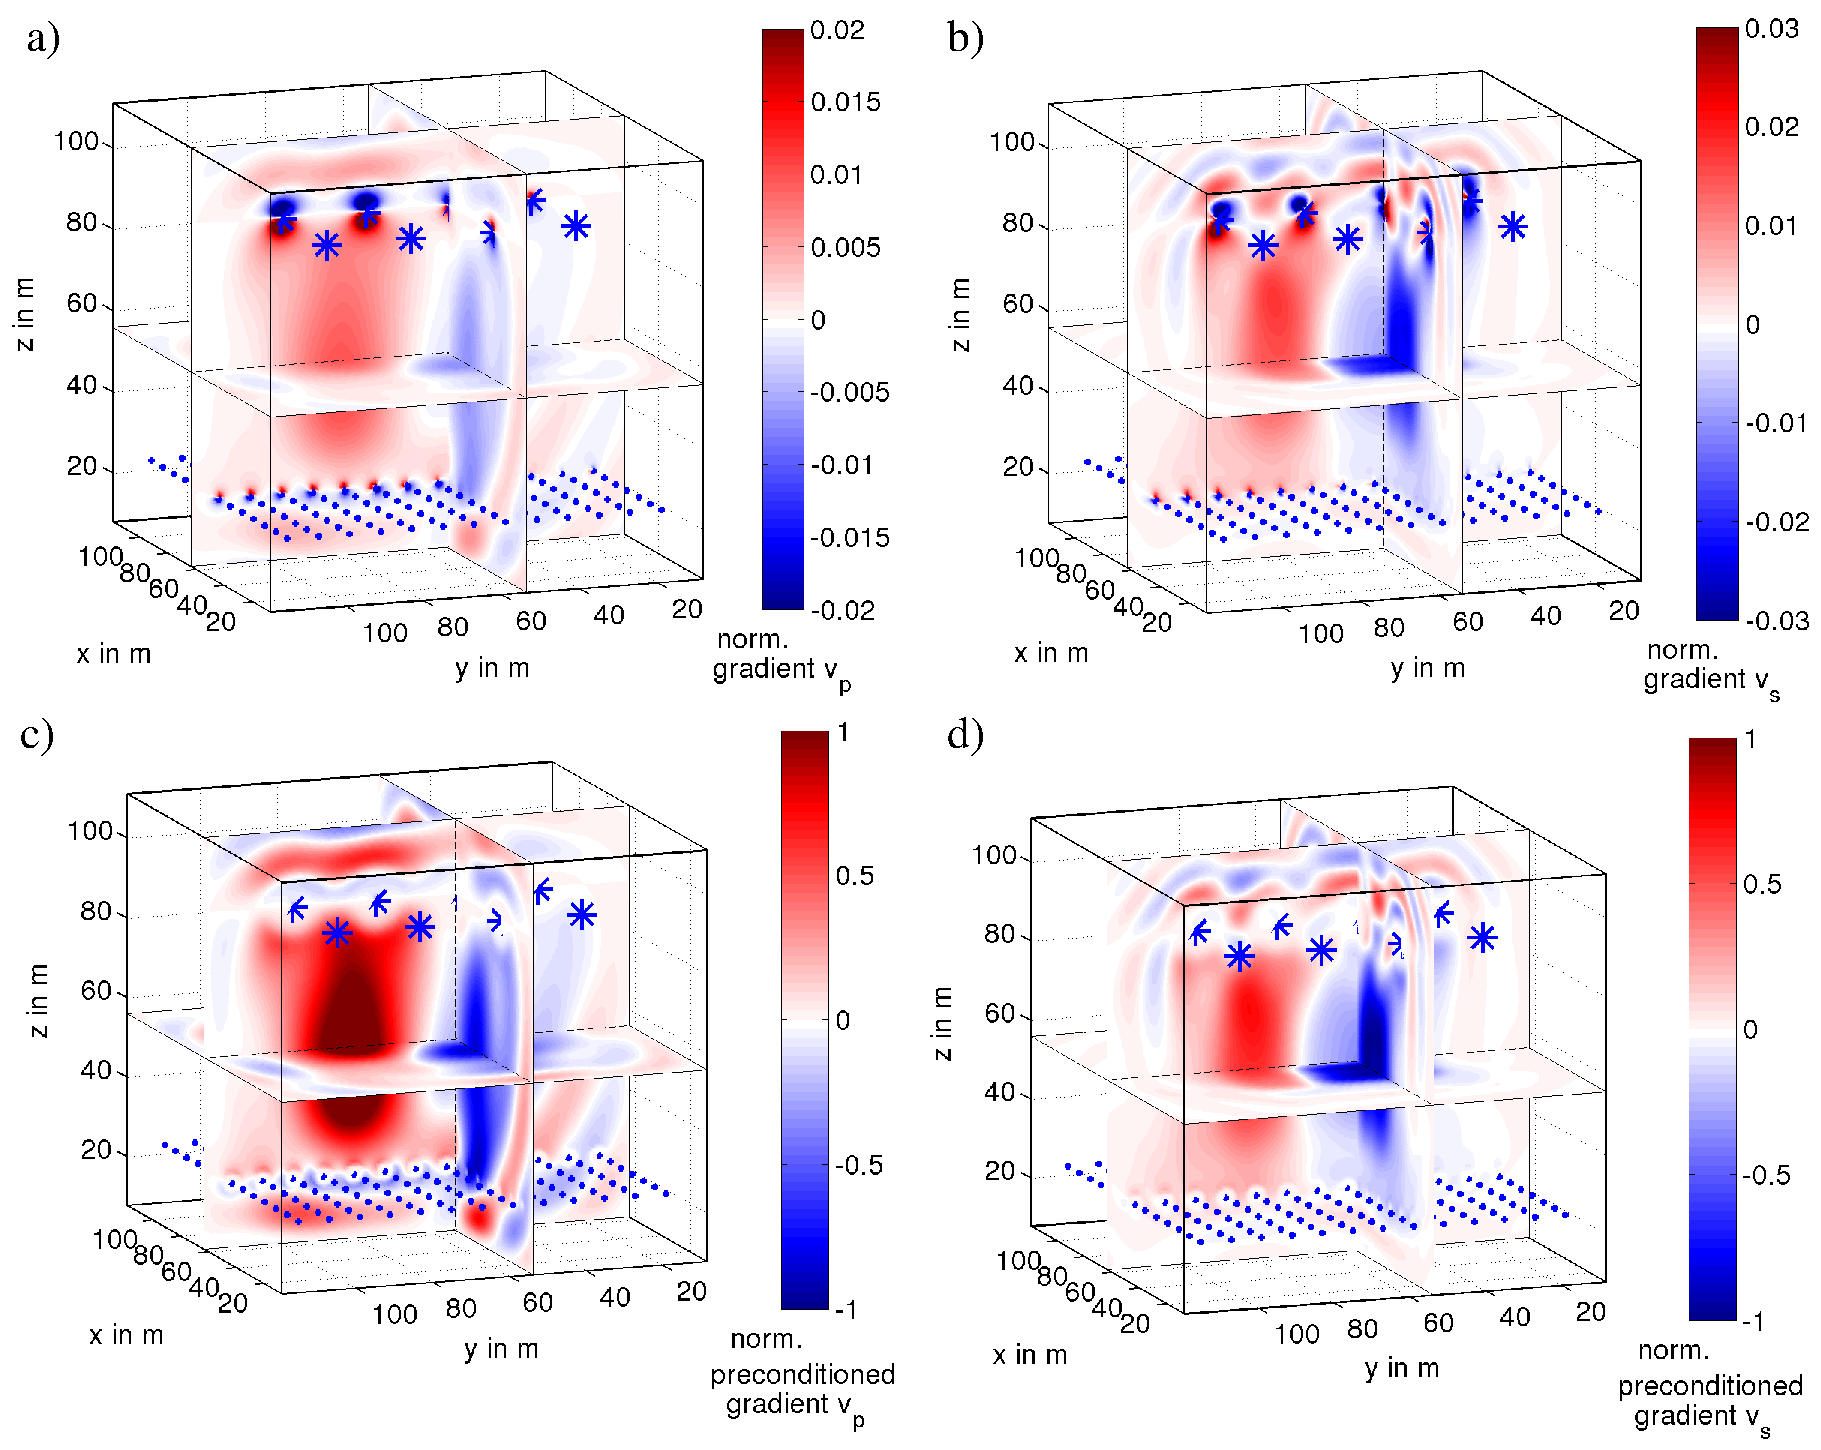
\includegraphics[width=\textwidth]{fig_toy/grad_toy}
\caption[Toy example - gradient before and after preconditioning]{Normalised gradients of first iteration : a) ``raw'' gradient $v_p$, b) ``raw'' gradient $v_s$, c) preconditioned gradient $v_p$ and d) preconditioned gradient $v_s$; sources (stars) and receivers (crosses) are indicated. }\label{fig:toy_grad}
\end{center}
\end{figure}
\subsection{Misfit and steplength proceedings}
The misfit and steplength values are stored in \textit{in\_and\_out/ifos3D\_invers.out}. They give insights into the proceedings of the inversion. After storing the values one in a row in textfiles, they can be plotted with the Matlab functions \textit{misfit\_toy.c} and \textit{steplength\_toy.c}. \\
The misfit proceedings are plotted in figure~\ref{fig:toy_misfit}. The values are normalised to the initial misfit. The curve shows a high convergence at the beginning of the inversion, where the rough model structures are included. The curve flattens as the inversion proceeds and only finer changes in the model are performed. Note, that with each new frequency stage data is added to the misfit and the misfit steps to higher values, which is then reduced within this stage.\\
\begin{figure}[h!]
\begin{center} 
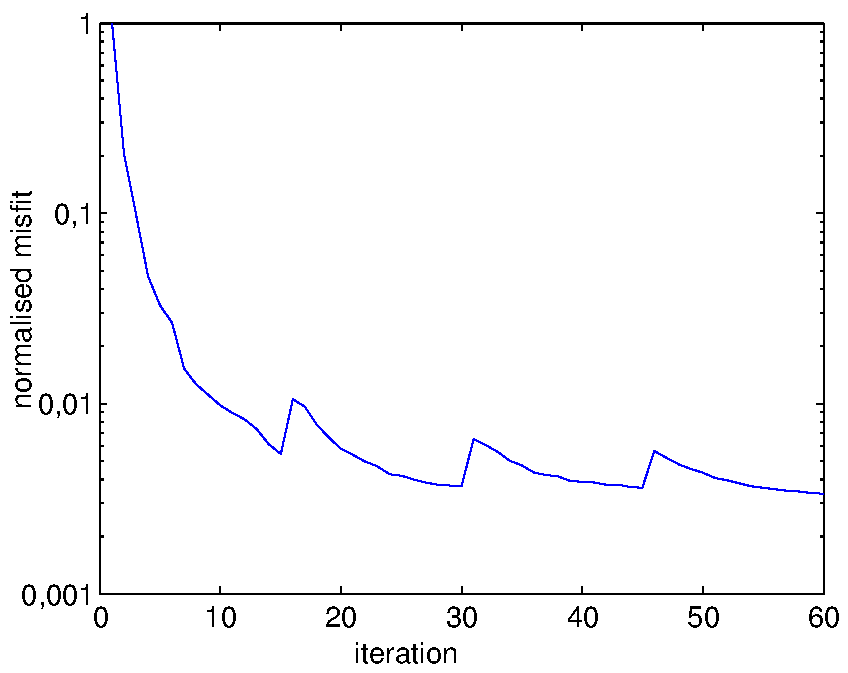
\includegraphics[width=0.7\textwidth]{fig_toy/toy_misfit}
\caption[Toy example - misfit]{Misfit normalised to initial value shows the convergence }\label{fig:toy_misfit}
\end{center}
\end{figure}
The steplength curve (figure~\ref{fig:toy_steplength}) shows a similar behaviour. At the beginning steplengths of few percent are found. That means the size of the model update is few percent of the average model parameter. These steplengths quickly decrease to less than 0.5\% after few iterations. Most model changes are thus made in the first few iterations whereas only the fine work is performed in the later iterations and at higher frequencies.
\begin{figure}[h!]
\begin{center}
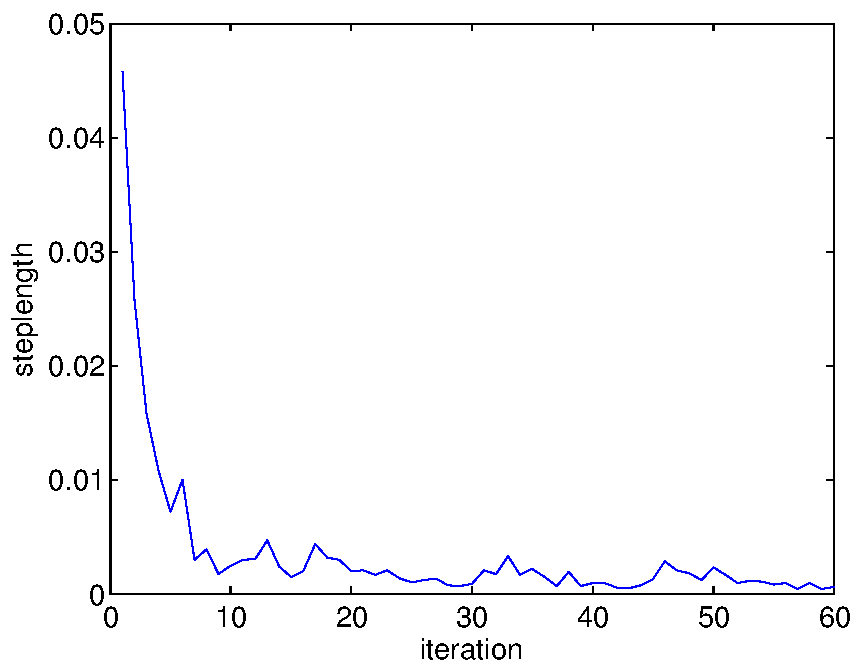
\includegraphics[width=0.7\textwidth]{fig_toy/toy_steplength}
\caption[Toy example - misfit]{Steplength proceedings}\label{fig:toy_steplength}
\end{center}
\end{figure}

\subsection{The final models}
Model parameters are written into the folder \textit{model} in each iteration for each parameter ($v_p$, $v_s$, $\rho$) in binary format (e.g. \textit{toy.vp\_it22}). They can be plotted similarly to the gradient with the program \textit{slice\_3D\_toy\_model.m}. Note, that gradient and model files share the same structure.\\
The results for the toy example is plotted for two 2D slices. Figure~\ref{fig:toy_result1} shows a horizontal slice through the box area. The three different box areas seen in the real model in a) and c) are well resolved for $v_p$ (b) and $v_s$ (d) after 60 iterations. However the $v_s$-model offers a clearly higher resolution due to the smaller wavelengths compared to the $v_p$-model. In transmission geometry a resolution down to one wavelength is possible and higher frequencies would be necessary to gain a better resolved box in $v_p$.
\begin{figure}[h!]
\begin{center}
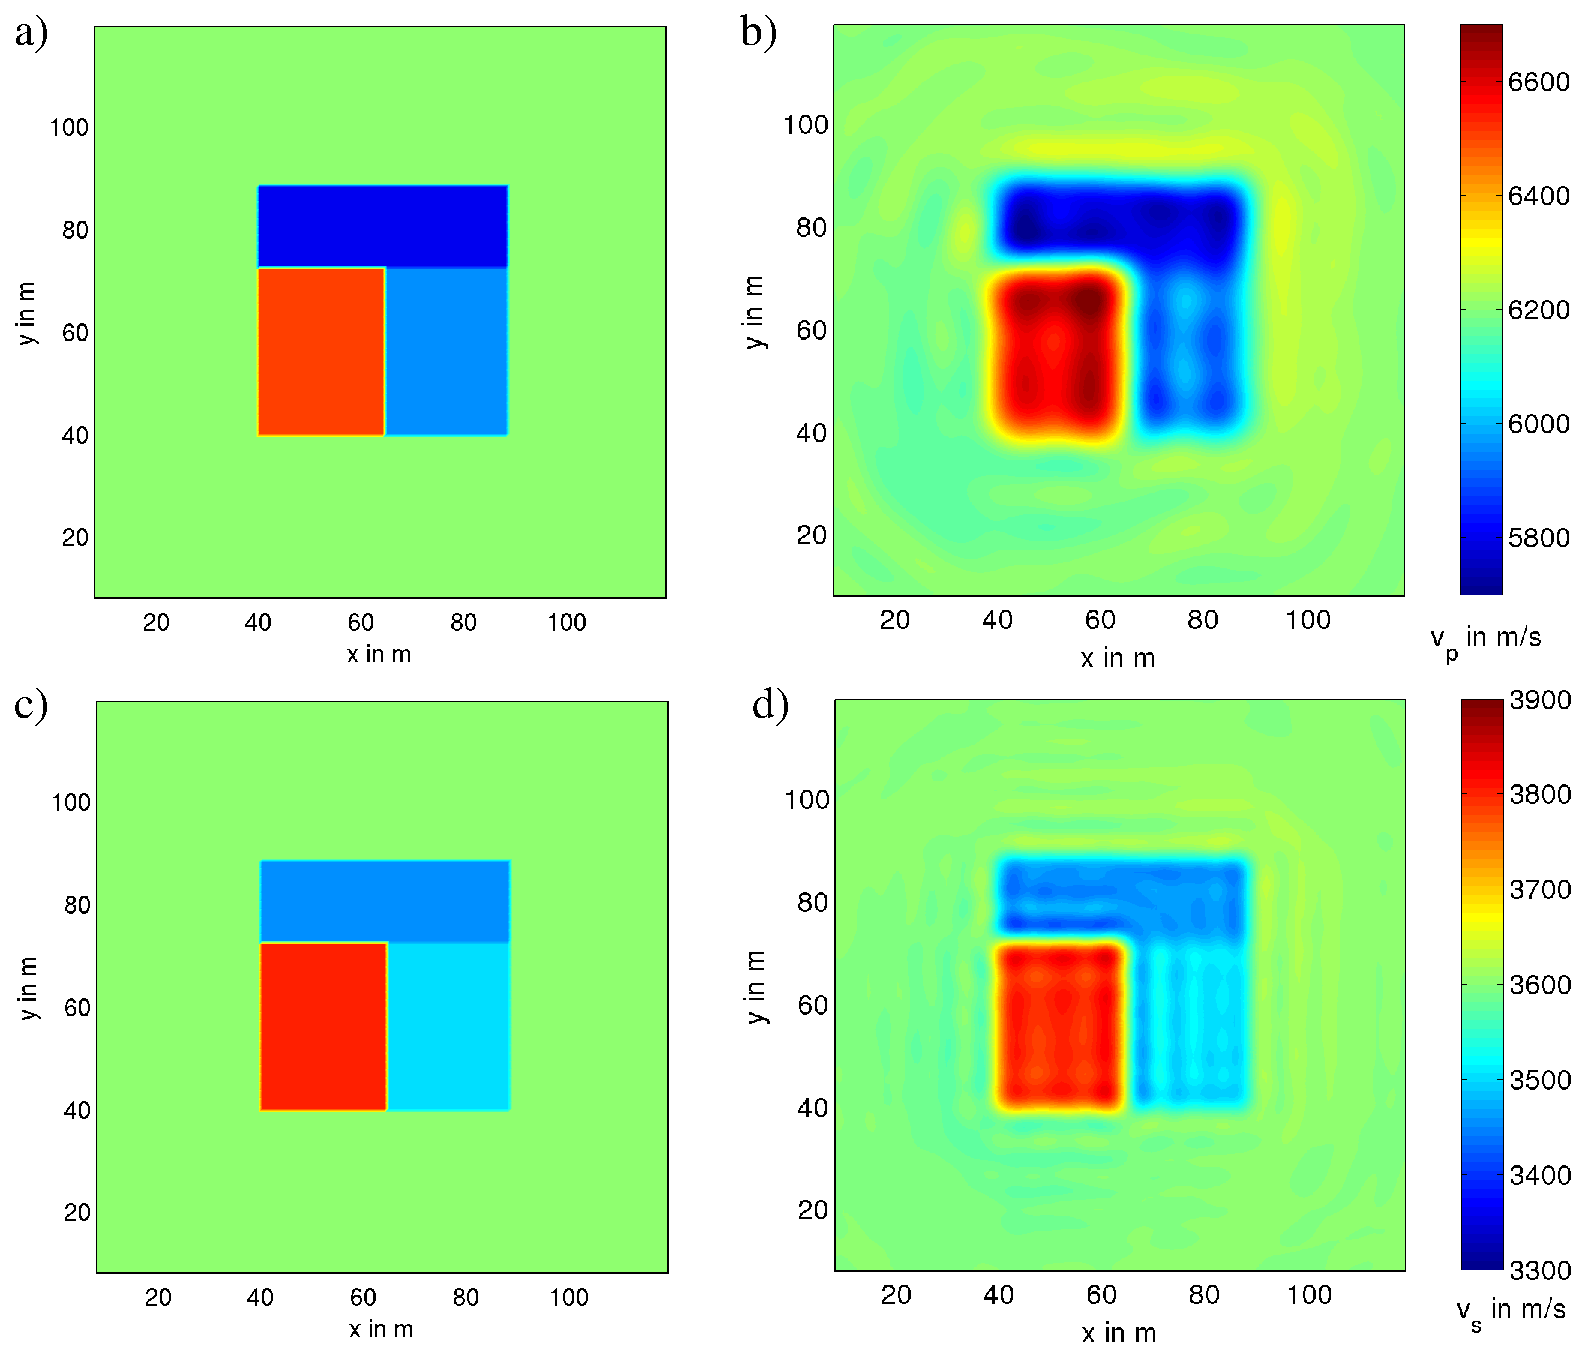
\includegraphics[width=\textwidth]{fig_toy/toy_model_result}
\caption[Toy example - final inverted models, horizontal slice]{Final inverted models (60 iteartions) compared to real models for horizontal slice at $z$=60\,m: a) real model $v_p$, b) inverted  model $v_p$, c) real model $v_s$ and d) inverted model $v_s$;  }\label{fig:toy_result1}
\end{center}
\end{figure}
A vertical slice of the models is plotted in figure~\ref{fig:toy_result2}. Overall, the vertical direction is more difficult to reconstruct, as can be ssen in the inverted models of $v_p$ (b) and $v_s$ (d) compared to the real models (a,b). The boundaries of the box are relatively well recovered for both parameters. The inversion of $v_p$ reconstructs the two main areas of the box, however the small high velocity area (dark red) cannot be resolved. This area is indicated in the inverted $v_s$ model, again showing the higher resolution of this parameter.
\begin{figure}[h!]
\begin{center}
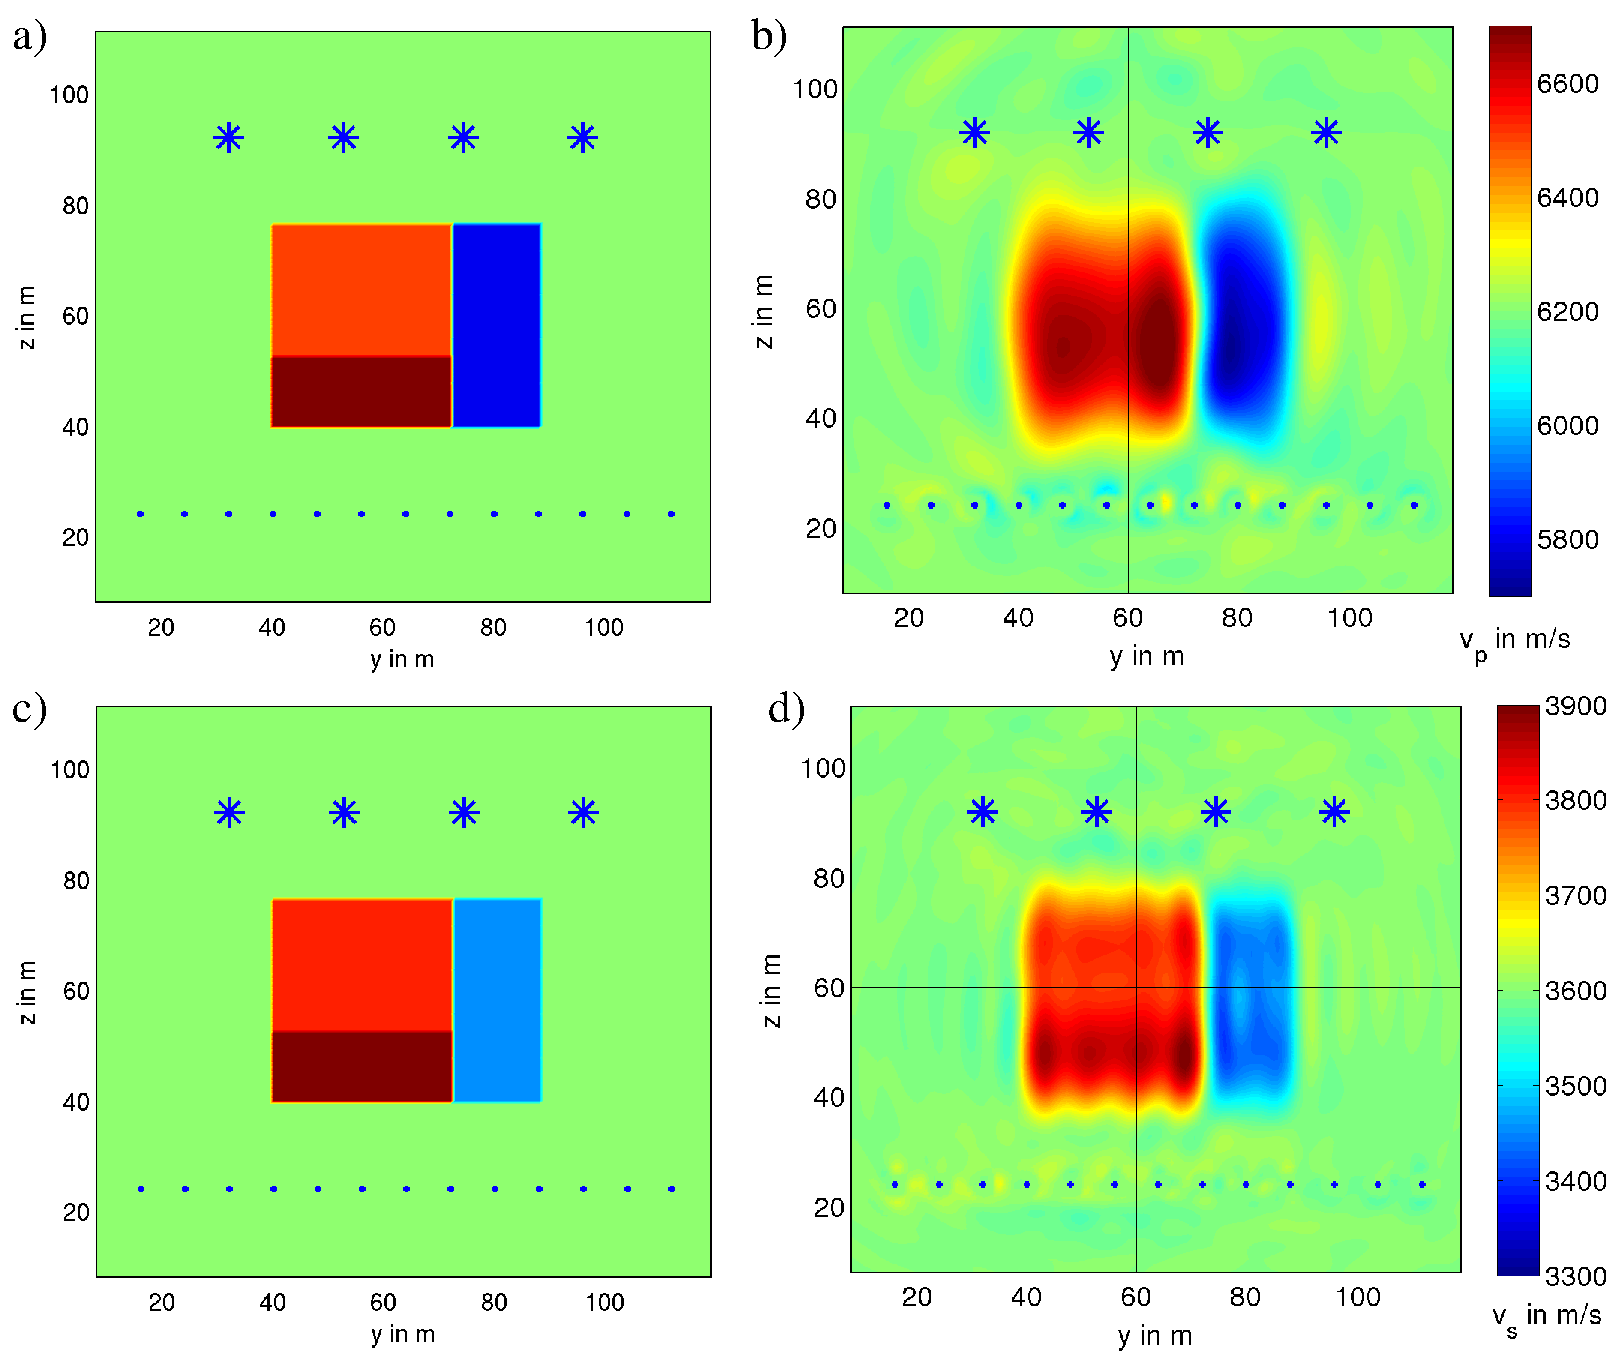
\includegraphics[width=\textwidth]{fig_toy/toy_model_result1}
\caption[Toy example - final inverted models, vertical slice]{Final inverted models (60 iterations) compared to real models for vertical slice at $x$=56\,m: a) real model $v_p$, b) inverted  model $v_p$, c) real model $v_s$ and d) inverted model $v_s$; }\label{fig:toy_result2}
\end{center}
\end{figure}

\section{Outlook}
This example is also included by \cite{But15}. Here the applications using the diagonal Hessian approximation and the L-BFGS method are shown. You can also look at the other applications \citep{But13, But15} which include the inversion of a random medium model in different transmission geonetries and a surface geometry model.


